% Template
\documentclass[dvipdfmx, 11pt]{beamer}

%%%% Packages %%%%%
%\usepackage{bxdpx-beamer}
%\usepackage{minijs}
%\usepackage{tabularx}
%\usepackage{graphicx}
% \usepackage{graphicx}
% \usepackage{amsmath,amssymb,amsthm}
% \usepackage{multirow}
\usepackage{multicol}
% \usepackage{url}
\usepackage{listings,jlisting}
\usepackage{tikz}
\usetikzlibrary{arrows,shapes}
\usetikzlibrary{positioning}


%%%% Fonts %%%%%
\renewcommand{\kanjifamilydefault}{\gtdefault}
 %\usepackage{otf} % otfパッケージ
\usepackage[deluxe]{otf} 
%\renewcommand{\kanjifamilydefault}{mg}
\usepackage{txfonts} % 数式・英文ローマン体を Lxfont にする
% \usepackage[T1]{fontenc} % 8bit フォント
% \usepackage{minijs}
% \usepackage{textcomp} % 欧文フォントの追加
% \usepackage[utf8]{inputenc} % 文字コードをUTF-8

%%%%% Beamer %%%%%
\usetheme{Madrid}
\useinnertheme{rectangles}
%\useoutertheme{smoothbars}
\setbeamercolor{enumerate}{fg=white, bg=black}
\usefonttheme{professionalfonts}
\setbeamertemplate{frametitle}[default][center]
\setbeamertemplate{navigation symbols}{}
% \setbeamercovered{transparent} % 好みに応じてどうぞ
\setbeamertemplate{footline}[frame number]
\setbeamercolor{page number in head/foot}{fg=black} % ページ数を表示する
% \setbeamerfont{footline}{size=\normalsize,series=\bfseries}
\setbeamerfont{footline}{size=\scriptsize,series=\mdseries}
\setbeamercolor{footline}{fg=black,bg=black}
\setbeamertemplate{blocks}[rounded][shadow=true]
\setbeamertemplate{items}[ball]
% \setbeamertemplate{enumerate items}[default]
% \setbeamerfont{alerted text}{series=\bfseries}
\newcommand{\backupbegin}{
   \newcounter{framenumberappendix}
   \setcounter{framenumberappendix}{\value{framenumber}}
}
\newcommand{\backupend}{
   \addtocounter{framenumberappendix}{-\value{framenumber}}
   \addtocounter{framenumber}{\value{framenumberappendix}} 
}
\renewcommand{\thefootnote}{\dag} % フットノート番号をダガーにする

%%%% Code %%%%%%%%%
\lstset{
 basicstyle=\ttfamily\color{black},
 keepspaces=true,
 escapechar=|,
 columns=[l]{fullflexible},
 commentstyle={\color{red}},
 stringstyle={\color{blue}},
}
%%%% My macro %%%%%
%%%%%%%%%%%%%%%%%%%%%%%%%%%%%%%%%%%%%%%%%%%%%%%%%%%%%%%%%%%%%%%%
% User-defined Macro
%%%%%%%%%%%%%%%%%%%%%%%%%%%%%%%%%%%%%%%%%%%%%%%%%%%%%%%%%%%%%%%%
\newcommand{\compress}{\itemsep0pt\parsep0pt\parskip0pt\partopsep0pt}
% \newcommand{\compress}{\itemsep1pt plus1pt\parsep0pt\parskip0pt}
% \newcommand{\code}[1]{\lstinline[basicstyle=\ttfamily]{#1}}
\newcommand{\gringo}{\textit{gringo}}
\newcommand{\clasp}{\textit{clasp}}
\newcommand{\clingo}{\textit{clingo}}
\newcommand{\teaspoon}{\textit{teaspoon}}
\newcommand{\sat}{\textsf{SAT}}
\newcommand{\unsat}{\textsf{UNSAT}}
% \newcommand{\web}[2]{\href{#1}{#2\ \raisebox{-0.15ex}{\beamergotobutton{Web}}}}
% \newcommand{\doi}[2]{\href{#1}{#2\ \raisebox{-0.15ex}{\beamergotobutton{DOI}}}}
% \newcommand{\weblink}[1]{\web{#1}{#1}}
% \newcommand{\imp}{\mathrel{\Rightarrow}}
% \newcommand{\Iff}{\mathrel{\Leftrightarrow}}
% \newcommand{\mybox}[1]{\fbox{\rule[.2cm]{0cm}{0cm}\mbox{${#1}$}}}
% \newcommand{\mycbox}[2]{\tikz[baseline]\node[fill=#1!10,anchor=base,rounded corners=2pt] () {#2};}
% \newcommand{\naf}[1]{\ensuremath{{\sim\!\!{#1}}}}
% \newcommand{\head}[1]{\ensuremath{\mathit{head}(#1)}}
% \newcommand{\body}[1]{\ensuremath{\mathit{body}(#1)}}
% \newcommand{\atom}[1]{\ensuremath{\mathit{atom}(#1)}}
% \newcommand{\poslits}[1]{\ensuremath{{#1}^+}}
% \newcommand{\neglits}[1]{\ensuremath{{#1}^-}}
% \newcommand{\pbody}[1]{\poslits{\body{#1}}}
% \newcommand{\nbody}[1]{\neglits{\body{#1}}}
% \newcommand{\Cn}[1]{\ensuremath{\mathit{Cn}(#1)}}
% \newcommand{\reduct}[2]{\ensuremath{#1^{#2}}}
% \newcommand{\OK}{\mbox{\textcolor{green}{\Pisymbol{pzd}{52}}}}
% \newcommand{\KO}{\mbox{\textcolor{red}{\Pisymbol{pzd}{56}}}}
% \newcommand{\code}[1]{\lstinline[basicstyle=\ttfamily]{#1}}
% \newcommand{\lw}[1]{\smash{\lower2.ex\hbox{#1}}}
\newcommand{\llw}[1]{\smash{\lower3.ex\hbox{#1}}}

\newenvironment{tableC}{%
  \scriptsize
  \renewcommand{\arraystretch}{0.9}
  \tabcolsep = 0.6mm
  % \begin{tabular}[t]{p{6mm}|rlr|rlr|rlr|rlr|rlr}\hline
  %   \multicolumn{1}{l|}{\llw{問題   }} &
  \begin{tabular}[t]{l|rlr|rlr|rlr|rlr|rlr}\hline
    \multicolumn{1}{l|}{\llw{問題}} &
    \multicolumn{3}{c|}{UD1} &
    \multicolumn{3}{c|}{UD2} &
    \multicolumn{3}{c|}{UD3} &
    \multicolumn{3}{c|}{UD4} &
    \multicolumn{3}{c}{UD5} \\
    & 
    \multicolumn{1}{c}{既知の} & & \multicolumn{1}{c|}{ASP} & 
    \multicolumn{1}{c}{既知の} & & \multicolumn{1}{c|}{ASP} & 
    \multicolumn{1}{c}{既知の} & & \multicolumn{1}{c|}{ASP} & 
    \multicolumn{1}{c}{既知の} & & \multicolumn{1}{c|}{ASP} & 
    \multicolumn{1}{c}{既知の} & & \multicolumn{1}{c}{ASP} \\
    & 
    ベスト & &  & 
    ベスト & &  & 
    ベスト & &  & 
    ベスト & &  & 
    ベスト & &  \\
    \hline
  }{%
    \hline
  \end{tabular}
}

\newcommand{\nodeVP}[3]{
  \coordinate[#2] (#1);
  \draw[fill=cyan!30] (#1)--+(-1,0)--+(0,1)--+(1,0)--cycle;
  \draw (#1)node[above]{\tiny{#3}};
  \draw[fill=black] (#1) +(-0.5,0.5)--+(0.5,0.5)--+(0,1)--cycle;
  \node[rectangle,above=0.5cm of #1,white](vp){\tiny{VP}};
  \coordinate[below=0.5cm of #1] (via_#1);
  \draw (via_#1)node[above right]{\tiny{[1..1]}};
  \draw (via_#1) +(170:0.2) arc (170:370:0.2);
  \draw (#1)--(via_#1);

}
\newcommand{\nodeTrans}[3]{
  \coordinate[#2] (#1);
  \draw[fill=cyan!30] (#1)--+(-1,0)--+(0,1)--+(1,0)--cycle;
  \draw (#1)node[above]{\tiny{#3}};
  \draw[fill=black] (#1) +(-0.5,0.5)--+(0.5,0.5)--+(0,1)--cycle;
  \node[rectangle,above=0.5cm of #1,white](vp){\tiny{VP}};
  \coordinate[below=1.7cm of #1] (via_#1);
  \draw (via_#1)node[below=0.2cm]{\tiny{[1..1]}};
  \draw (via_#1) +(135:0.2) arc (135:405:0.2);
  \draw (#1)--(via_#1);

}

\newcommand{\nodeVPdashed}[3]{
  \coordinate[#2] (#1);
  \draw[fill=cyan!30,dashed] (#1)--+(-1,0)--+(0,1)--+(1,0)--cycle;
  \draw (#1)node[above]{\tiny{#3}};
  \fill[black] (#1) +(-0.5,0.5)--+(0.5,0.5)-- +(0,1)--cycle;
  \node[rectangle,above=0.5cm of #1,white](vp){\tiny{VP}};
  \coordinate[below=0.5cm of #1] (via_#1);
  \draw (via_#1)node[above right]{\tiny{[1..1]}};
  \draw (via_#1) +(-0.2,0) arc (180:360:0.2);
  \draw (#1)--(via_#1);

}

\newcommand{\nodeV}[4]{
  \node [draw,inner xsep=2pt,#2,fill=black!10,font=\tiny] (#1){
      \begin{tabular}{l}
       #3\\
       #4\\
      \end{tabular}
  };
  \fill [black] (#1.north west)--++(0,-2mm)--++(1mm,0)--++(1mm,0)--++(0,2mm); 
  \draw (#1.north west) ++(1mm,-1mm) node[white]{\tiny{v}};
}

\newcommand{\nodeVchoiced}[4]{
  \node [draw,inner xsep=2pt,#2,fill=red!50,font=\tiny] (#1){
      \begin{tabular}{l}
       #3\\
       #4\\
      \end{tabular}
  };
  \fill [black] (#1.north west)--++(0,-2mm)--++(1mm,0)--++(1mm,0)--++(0,2mm); 
  \draw (#1.north west) ++(1mm,-1mm) node[white]{\tiny{v}};

}


%%%%%%%%%%%%%%%%%%%%%%%%%%%%%%%%%%%%%%%%%%%%%%%%%%%%
\title{解集合プログラミングを用いた\\多目的車両装備仕様問題の解法}
\author{竹内頼人}
\institute{名古屋大学 大学院情報学研究科 番原研究室}
\date{2020年度番原研中間発表\\ 2020年12月11日}
\begin{document}
\frame{\titlepage}
%%%%%%%%%%%%%%%%%%%%%%%%%%%%%%%%%%%%%%%%%%%%%%%%%%%%
\begin{frame}{車両装備仕様問題}
 \structure{\bf 車両装備仕様}とは,簡単に言うと,自動車のカタログに記載されている
 \textbf{モデル/グレードと装備の一覧表}のことである.
 \begin{itemize}
  \item 車両の装備を決定するために,
	現状では専門知識をもつ技術者の多大な労力が費やされている.
  \item 装備仕様決定の自動化・効率化は自動車メーカーにとって重要な課題の一つである.
 \end{itemize}
 \begin{block}{車両装備仕様問題 (組合せ最適化問題の一種)}
  \begin{itemize}
   \item 装備タイプと装備オプションに対する
	 \structure{\bf 範囲制約},
	 \structure{\bf 依存制約},
	 \structure{\bf 燃費制約}
	 から構成される.
   \item {\bf 予想販売台数が最大}となる装備仕様を求めることが目的である.
  \end{itemize}
 \end{block}
 \begin{alertblock}{CAFE基準(企業別平均燃費基準)}
  \begin{itemize}
   \item 車種別ではなくメーカー全体での出荷台数を加味した平均燃費を算出し,
	 規制をかける方式
   \item 燃費制約としてCAFE基準を用いた問題を,\structure{\bf CAFE問題}と呼ぶ.
  \end{itemize}
 \end{alertblock}
\end{frame}
%%%%%%%%%%%%%%%%%%%%%%%%%%%%%%%%%%%%%%%%%%%%%%%%%%%%
\begin{frame}{CAFE問題の例}
  \begin{columns}
    \begin{column}{0.75\linewidth}
      \scalebox{0.8}[0.8]{ 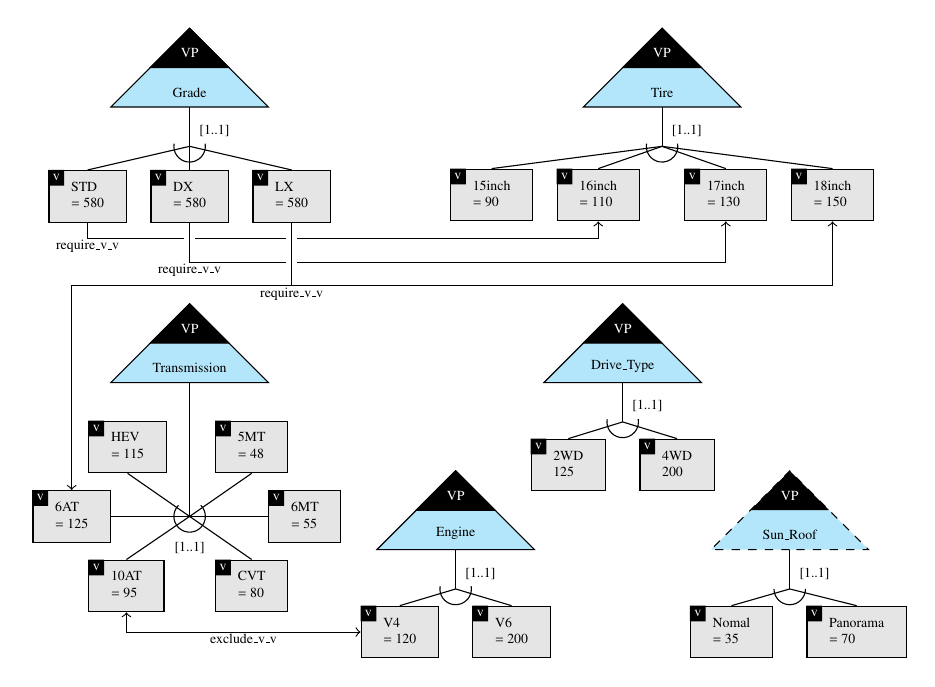
\begin{tikzpicture}
 % Grade
  \nodeVP{grade}{at={(0,0)}}{Grade};
  \nodeV{dx}{below=0.3cm of via_grade}{DX}{= 580};
  \draw(via_grade)--(dx.north);
  \nodeV{std}{left=0.3cm of dx}{STD}{= 580};
  \draw(via_grade)--(std.north);
  \nodeV{lx}{right=0.3cm of dx}{LX}{= 580};
  \draw(via_grade)--(lx.north);

  % Tire
  \nodeVP{tire}{right=6cm of grade}{Tire};
  \nodeV{16inch}{below left=0.4cm of via_tire}{16inch}{= 110};
  \nodeV{17inch}{below right=0.4cm of via_tire}{17inch}{= 130};
  \nodeV{15inch}{left=0.3cm of 16inch}{15inch}{= 90};
  \nodeV{18inch}{right=0.3cm of 17inch}{18inch}{= 150};
  \draw (via_tire)--(15inch.north);
  \draw (via_tire)--(16inch.north);
  \draw (via_tire)--(17inch.north);
  \draw (via_tire)--(18inch.north);

  % Transmission
  \nodeTrans{trans}{below=3.5cm of grade}{Transmission};
  \nodeV{6at}{left=1cm of via_trans}{6AT}{= 125};
  \nodeV{hev}{above right=0.3cm of 6at.north}{HEV}{= 115};
  \nodeV{10at}{below right=0.3cm of 6at.south}{10AT}{= 95};
  \nodeV{6mt}{right=1cm of via_trans}{6MT}{= 55};
  \nodeV{5mt}{above left=0.3cm of 6mt.north}{5MT}{= 48};
  \nodeV{cvt}{below left=0.3cm of 6mt.south}{CVT}{= 80};
  \draw (via_trans)--(10at.north);
  \draw (via_trans)--(6at.east);
  \draw (via_trans)--(hev.south);
  \draw (via_trans)--(6mt.west);
  \draw (via_trans)--(5mt.south);
  \draw (via_trans)--(cvt.north);

  % Drive_Type
  \nodeVP{drivetype}{right=5.5cm of trans}{Drive\_Type};
  \nodeV{2wd}{below left=0.3cm of via_drivetype}{2WD}{125};
  \draw (via_drivetype)--(2wd.north);
  \nodeV{4wd}{below right=0.3cm of via_drivetype}{4WD}{200};
  \draw (via_drivetype)--(4wd.north);


  % Sun_Roof
  \nodeVPdashed{sunroof}{below right=3cm of drivetype}{Sun\_Roof};
  \nodeV{nomal}{below left=0.3cm of via_sunroof}{Nomal}{= 35};
  \draw (via_sunroof)--(nomal.north);
  \nodeV{panorama}{below right=0.3cm of via_sunroof}{Panorama}{= 70};
  \draw (via_sunroof)--(panorama.north);

  % Engine
  \nodeVP{engine}{below left=3cm of drivetype}{Engine};
  \nodeV{v4}{below left=0.3cm of via_engine}{V4}{= 120};
  \draw (via_engine)--(v4.north);
  \nodeV{v6}{below right=0.3cm of via_engine}{V6}{= 200};
  \draw (via_engine)--(v6.north);
  
 

  % require
  \draw[->] (std.south)--++(0,-0.2) node[below=-1mm] {\tiny{require\_v\_v}} -|(16inch.south);
  \draw[white,line width=4pt](dx.south) ++(0,-0.1)--++(0,-0.5);
  \draw[->] (dx.south)--++(0,-0.5) node[below=-1mm] {\tiny{require\_v\_v}} -|(17inch.south);
  \draw[white,line width=4pt] (lx.south) ++(0,-0.1)--++(0,-0.8);
  \draw[->] (lx.south)--++(0,-0.8) node[below=-1mm] {\tiny{require\_v\_v}} -|(18inch.south);
  \draw[->] (lx.south)--++(0,-0.8) -|(6at.north);

  % exclude
  \draw[<->] (v4.west)-|(10at.south) node[pos=0.25,below=-1mm]{\tiny{exclude\_v\_v}};
 \end{tikzpicture}
}
      \uncover<2>{
      \begin{exampleblock}{}\centering
        STD,DX,LXグレードの3車種を生産するとする.
      \end{exampleblock}}
    \end{column}
    \begin{column}{0.25\linewidth}
      \begin{footnotesize}
        \begin{itemize}
        \item プロダクトライン開発で用いられる可変性モデルによって記述
        \item 6個の装備タイプ,19個の装備オプション
        \item 各タイプの選択可能なオプション数はすべて1
        \item 各オプションの数字はIWR値と呼ばれ,直観的にはその重量
        \item 5個の依存制約
        \item \textsf{Sun Roof}以外は必須タイプ
        \end{itemize}
      \end{footnotesize}
    \end{column}
  \end{columns}
\end{frame}
%%%%%%%%%%%%%%%%%%%%%%%%%%%%%%%%%%%%%%%%%%%%%%%%%%%%
\begin{frame}{CAFE問題の解 {\normalsize (CAFE基準値: 8.5km/L)}}\small
 \begin{exampleblock}{解の例}
  \centering
  \renewcommand{\arraystretch}{0.9}
  %\tabcolsep = 5mm
  \begin{tabular}{p{10mm}|p{25mm}|p{15mm}|p{15mm}|p{15mm}} 
   \multicolumn{2}{l|}{装備仕様}  & 車種1 & 車種2 & 車種3 \\\hline
   装備 & Grade  & \ STD & \ DX  & \ LX\\
   &Drive\_Type  & \ 2WD    & \ 2WD    & \ 4WD\\
   &Engine	     & \ V6      & \ V6     & \ V6\\
   &Tire	     & \ 16inch & \ 17inch & \ 18inch\\
   &Transmission & \ 6AT     & \ HEV     & \ 10AT\\
   &Sun\_Roof    & \ -               & \ -   & \ -  
  \end{tabular}
 \end{exampleblock}

 \pause

 \begin{block}{}
  \centering
  \renewcommand{\arraystretch}{0.9}
  %\tabcolsep = 5mm
  \begin{tabular}{p{38mm}|p{15mm}|p{15mm}|p{15mm}} 
   IWR 値の総和           & 1,130  & 1,130   & 1,255 \\ %\hline
   燃費(km/L)      & 8.8  & 8.8     & 8.0 \\ %\hline
   予想販売台数    & 2,007   & 2,007   & 1,511  \\ \hline
   平均燃費(km/L)  & \multicolumn{3}{c}{8.5} \\ 
   予想販売台数(合計)  & \multicolumn{3}{c}{5,525} 
  \end{tabular}
 \end{block}

 \vfill
 \begin{itemize}
 \item 車種3ではCAFE基準値を下回っているが,平均燃費は8.5km/Lとなり,
       燃費制約を満たしている.
 \end{itemize}
\end{frame}
%%%%%%%%%%%%%%%%%%%%%%%%%%%%%%%%%%%%%%%%%%%%%%%%%%%%
\begin{frame}{解集合プログラミング(Answer Set Programming; ASP)}
 \begin{itemize}
 \item \structure{\bf ASPの言語}は,一階論理に基づく知識表現言語の一種である.
 %\item \structure{\bf ASPのプログラム}は,ASPルールの有限集合である.
 \item \structure{\bf ASPシステム}は,安定モデル意味論~[Gelfond and Lifschitz '88]
   に基づく解集合を計算するシステムである.
 \item 近年,SAT技術を利用した高速なASPシステムが開発され,
   ロボット工学,システム検証,システム生物学
   など様々な分野への実用的応用が急速に拡大している.
 \end{itemize}
\vfill
 \begin{alertblock}{CAFE問題に対してASPを用いる利点}
   \begin{itemize} 
    \item ASP言語の高い表現力により,各種制約を簡潔に記述できる.
%    \item 高速なASPシステムを利用できる.
    \item 解の最適性を保証でき,最適解の列挙も可能である.
    \item ASPソルバー{\it asprin} では,複数の目的関数に対する
	  辞書式最適化やパレート最適化など,柔軟な最適値探索が可能である.
   \end{itemize}
 \end{alertblock}
\end{frame}
%%%%%%%%%%%%%%%%%%%%%%%%%%%%%%%%%%%%%%%%%%%%%%%%%%%%
\begin{frame}{研究の目的と内容}
  \begin{alertblock}{目的}
    ASP技術を用いて,CAFE問題を効率よく解くシステムを設計・実装し,
    実用規模の問題で評価する.
  \end{alertblock}
\begin{block}{研究内容}
 \begin{itemize}
  \item CAFE問題を解くASP符号化を2種類考案
	\begin{itemize}
	 \item 基本符号化
	 \item 改良符号化
	\end{itemize}
  \item 企業から提供された実データを用いた評価実験
	\begin{itemize}
	 \item 小規模な問題に対して,最適解を全列挙することができた.
	 \item 実用規模,およびより大規模な問題に対して,改良符号化の優位性が確認できた.
	\end{itemize}
  \item \structure{目的関数に装備オプション数の最小化を追加し,
	{\bf 多目的車両装備仕様問題}へ拡張}
	\begin{itemize}
	 \item 2種類の最適化方法を実装・評価
	       (\structure{\bf 辞書式最適化},\structure{\bf パレート最適化})
	\end{itemize}
 \end{itemize}
\end{block}  
\end{frame}
%%%%%%%%%%%%%%%%%%%%%%%%%%%%%%%%%%%%%%%%%%%%%%%%%%%%
\begin{frame}{多目的車両装備仕様問題}
 \begin{itemize}
  \item 製造ラインの削減や,大量生産を促進することを狙いとして,
	{\bf 予想販売台数の最大化}に加えて,{\bf 装備オプション数の最小化}も可能なように
	拡張された車両装備仕様問題
 \end{itemize}
%  \begin{alertblock}{}
%   複数の目的関数をもつ車両装備仕様問題
%  \end{alertblock}

% \begin{block}{多目的CAFE問題}
%  \begin{itemize}
%   \item 目的関数
% 	\begin{itemize}
% 	 \item 予想販売台数の最大化
% 	 \item 装備オプション数の最小化
% 	\end{itemize}
%   \item 燃費制約
% 	\begin{itemize}
% 	 \item CAFE基準
% 	\end{itemize}
%  \end{itemize}
% \end{block}
 \begin{block}{最適化方法}
  \begin{enumerate}
   \item \structure{\bf 辞書式最適化}
	 \begin{itemize}
	  \item 予想販売台数の最大化,装備オプション数の最小化の順に最適化を行う.
	 \end{itemize}
   \item \structure{\bf パレート最適化}
	 \begin{itemize}
	  \item 目的関数に優先度をつけず,トレードオフな解(パレート解)を列挙する.
	 \end{itemize}
  \end{enumerate}
 \end{block}

\end{frame}
%%%%%%%%%%%%%%%%%%%%%%%%%%%%%%%%%%%%%%%%%%%%%%%%%%%%
\begin{frame}{辞書式最適化}
 \begin{itemize}
  \item CAFE基準値は8.5km/Lとする.
 \end{itemize}
 \begin{exampleblock}{}
  \tiny
  \centering
    \begin{tabular}{l|l|c|c|c||c|c|c||c|c|c} 
    \multicolumn{2}{l|}{} & \multicolumn{3}{c||}{解1} & \multicolumn{3}{c||}{解2} & \multicolumn{3}{c}{\bf{解3}}\\ \hline
    \multicolumn{2}{l|}{装備仕様} & 1 & 2 & 3 & 1 & 2 & 3 & 1 & 2 & 3 \\ \hline
    装備 & \textsf{Grade}        & \textsf{STD}& \textsf{DX} & \textsf{LX}& \textsf{STD} & \textsf{DX}  & \textsf{LX}    & \textsf{STD} & \textsf{DX}  & \textsf{LX}       \\
        & \textsf{Drive\_Type}  & \textsf{4WD}  & \textsf{2WD} & \textsf{4WD} & \textsf{2WD} & \textsf{2WD} & \textsf{4WD} & \textsf{2WD} & \textsf{2WD} & \textsf{4WD}  \\
        & \textsf{Engine} & \textsf{V4} & \textsf{V6} & \textsf{V6} & \textsf{V6} & \textsf{V6} & \textsf{V6} & \textsf{V6} & \textsf{V6} & \textsf{V6}      \\ 
        & \textsf{Tire} & \textsf{16}	& \textsf{17} & \textsf{18} & \textsf{16}  & \textsf{17}  & \textsf{18} & \textsf{16} & \textsf{17} & \textsf{18} \\
        & \textsf{Transmission} & \textsf{5MT} & \textsf{HEV} & \textsf{10AT} & \textsf{CVT} & \textsf{HEV} & \textsf{10AT}  & \textsf{6AT} & \textsf{HEV} & \textsf{10AT}     \\
        & \textsf{Sun\_Roof} & \textsf{Panorama} & -   & -       & \textsf{Nomal} & -  & -     & -   & -   & -       \\ \hline
    \multicolumn{2}{l|}{IWR値の総和}  & 1,128 & 1,130   & 1,255    & 1,130 & 1,130&1,255  & 1,130& 1,130& 1,255     \\ %\hline
    \multicolumn{2}{l|}{燃費(km/L)}    & 8.9 & 8.8    & 8.0     & 8.8 & 8.8  & 8.0 & 8.8  & 8.8  & 8.0         \\ %\hline
    \multicolumn{2}{l|}{予想販売台数}  & 2,007  & 2,007   & 1,511   & 2,007 & 2,007 & 1,511 & 2,007& 2,007& 1,511       \\ \hline
    \multicolumn{2}{l|}{平均燃費(km/L)} & \multicolumn{3}{c||}{8.6} & \multicolumn{3}{c||}{8.5} & \multicolumn{3}{c}{8.5}\\ 
    \multicolumn{2}{l|}{予想販売台数(合計)}  & \multicolumn{3}{c||}{5,525} & \multicolumn{3}{c||}{5,525}  &\multicolumn{3}{c}{5,525}\\
    \multicolumn{2}{l|}{オプション数}  & \multicolumn{3}{c||}{14} & \multicolumn{3}{c||}{13}  &\multicolumn{3}{c}{12}\\ 
  \end{tabular}
 \end{exampleblock}
 \begin{itemize}
  \item 予想販売台数最大化のみの単目的最適化では,
	予想販売台数が5,525台である最適解が(解1,解2,解3)の3つ存在する.
  \item 装備オプション数最小化を加えた辞書式最適化では,
	得られる最適解はオプション数が最も小さい(解3)のただ1つだけとなる.
 \end{itemize}
 \begin{alertblock}{}
  目的関数に優先度をつけ,解が複数存在するときに優劣をつけることが可能
 \end{alertblock}
\end{frame}
%%%%%%%%%%%%%%%%%%%%%%%%%%%%%%%%%%%%%%%%%%%%%%%%%%%%
% \begin{frame}{パレート最適解の全列挙(案1)}
%  \begin{exampleblock}{}
%   \centering
%   \tiny
%   \begin{tabular}{l|l|c|c|c||c|c|c}
%    \multicolumn{2}{l|}{} & \multicolumn{3}{c||}{解1} & \multicolumn{3}{c}{解2}\\ \hline
%    \multicolumn{2}{l|}{装備仕様} & 1 & 2 & 3 & 1 & 2 & 3 \\ \hline
%    装備 & Grade & STD & DX & LX & STD & DX & LX \\
%        & Drive\_Type & 2WD & 2WD & 4WD & 2WD & 2WD & 4WD\\
%        & Engine & V6 & V6 & V6 & V6 & V6 & V6 \\
%        & Tire & 16 & 17 & 18 & 16 & 17 & 18 \\
%        & Transmission & 6AT & HEV & 10AT & 10AT & HEV & 10AT \\
%        & Sun\_Roof & - & - & - & - & - & - \\ \hline
%    \multicolumn{2}{l|}{予想販売台数(合計)}  & \multicolumn{3}{c||}{5,525} & \multicolumn{3}{c}{5,475} \\ 
%    \multicolumn{2}{l|}{オプション数}  & \multicolumn{3}{c||}{12} & \multicolumn{3}{c}{11} \\
%    \multicolumn{8}{c}{}
%   \end{tabular}
%   \begin{tabular}{l|l|c|c|c||c|c|c}
%    \multicolumn{2}{l|}{} & \multicolumn{3}{c||}{解3} & \multicolumn{3}{c}{解4}\\ \hline
%    \multicolumn{2}{l|}{装備仕様} & 1 & 2 & 3 & 1 & 2 & 3 \\ \hline
%    装備 & Grade & STD & DX & LX & STD & DX & LX \\
%        & Drive\_Type & 2WD & 2WD & 2WD & 2WD & 2WD & 2WD\\
%        & Engine & V6 & V6 & V6 & V6 & V6 & V6 \\
%        & Tire & 16 & 17 & 18 & 16 & 17 & 18 \\
%        & Transmission & 10AT & HEV & 10AT & 10AT & 10AT & 10AT \\
%        & Sun\_Roof & - & - & - & - & - & - \\ \hline
%    \multicolumn{2}{l|}{予想販売台数(合計)}  & \multicolumn{3}{c||}{5,135} & \multicolumn{3}{c}{4,723} \\ 
%     \multicolumn{2}{l|}{オプション数}  & \multicolumn{3}{c||}{10} & \multicolumn{3}{c}{9} \\
   
%   \end{tabular}
%  \end{exampleblock}
% \end{frame}
% %%%%%%%%%%%%%%%%%%%%%%%%%%%%%%%%%%%%%%%%%%%%%%%%%%%%
\begin{frame}{パレート最適化}
 \begin{itemize}
  \item CAFE基準値は8.5km/Lとする.
 \end{itemize}
 \begin{exampleblock}{}
  \centering
  \tiny
  \tabcolsep=1.5mm
  \begin{tabular}{l|l|c|c|c||c|c|c||c|c|c||c|c|c}
   \multicolumn{2}{l|}{} & \multicolumn{3}{c||}{解1} & \multicolumn{3}{c||}{解2} & \multicolumn{3}{c||}{解3} & \multicolumn{3}{c}{解4}\\ \hline
   \multicolumn{2}{l|}{装備仕様} & 1 & 2 & 3 & 1 & 2 & 3 & 1 & 2 & 3 & 1 & 2 & 3 \\ \hline
   装備 & Grade & STD & DX & LX & STD & DX & LX & STD & DX & LX & STD & DX & LX \\
       & Drive\_Type & 2WD & 2WD & \alert{4WD} & 2WD & 2WD & \alert{4WD} & 2WD & 2WD & \alert{2WD} & 2WD & 2WD & \alert{2WD}\\
       & Engine & V6 & V6 & V6 & V6 & V6 & V6 & V6 & V6 & V6 & V6 & V6 & V6 \\
       & Tire & 16 & 17 & 18 & 16 & 17 & 18 & 16 & 17 & 18 & 16 & 17 & 18 \\
       & Transmission & \alert{6AT} & \alert{HEV} & 10AT & \alert{10AT} & \alert{HEV} & 10AT & \alert{10AT} & \alert{HEV} & 10AT & \alert{10AT} & \alert{10AT} & 10AT \\
       & Sun\_Roof & - & - & - & - & - & - & - & - & - & - & - & - \\ \hline
   \multicolumn{2}{l|}{予想販売台数(合計)}  & \multicolumn{3}{c||}{\bf 5,525} & \multicolumn{3}{c||}{\bf 5,475} & \multicolumn{3}{c||}{\bf 5,135} & \multicolumn{3}{c}{\bf 4,723} \\ 
   \multicolumn{2}{l|}{オプション数} & \multicolumn{3}{c||}{\bf 12} & \multicolumn{3}{c||}{\bf 11} & \multicolumn{3}{c||}{\bf 10} & \multicolumn{3}{c}{\bf 9} \\
   \multicolumn{14}{c}{}
  \end{tabular}
 \end{exampleblock}
 \begin{itemize}
  \item 4つのパレート解が得られ,それぞれトレードオフな関係になっていることがわかる.
 \end{itemize}
 \begin{alertblock}{}
  これらのパレート解からユーザの選好に合う解を選ぶことができ,
  柔軟な意思決定が可能
 \end{alertblock}
\end{frame}
%%%%%%%%%%%%%%%%%%%%%%%%%%%%%%%%%%%%%%%%%%%%%%%%%%%%
\begin{frame}{まとめ}
ASPを用いたCAFE問題ソルバーの設計・実装について述べた.
\begin{alertblock}{開発したCAFE問題ソルバーの特長}
   \begin{itemize}
   \item \structure{\bf 記述性: }
	 ASPの表現力の高さを活かし,CAFE問題の制約を簡潔に記述できる.
   \item \structure{\bf 効率性: }
	 改良符号化を用いることで,大規模な問題にも適用可能である.
   \item \structure{\bf 拡張性: }
	 多目的車両装備仕様問題にも適用可能で,ユーザの選好に合わせて
	 目的関数の追加や最適化方法の選択が柔軟にできる.
   \end{itemize}
\end{alertblock}
\begin{block}{今後の課題}
\begin{itemize}
\item 装備に関する制約は,まず企画部門で設定され,開発部門,生産部門,
  販売部門に受け渡され,各部門で制約が追加されながら徐々に成
  熟していく.
\item さらなる制約(例:ZEV規制)を実装することにより,CAFE問題ソルバーを拡張する
  ことが今後の課題である.
\end{itemize}
 
\end{block}
\end{frame}
\begin{frame}{発表歴}
 \begin{itemize}
  \item 2020/9/3 NII共同研究 第1回研究会合
  \item 2020/9/9 日本ソフトウェア科学会 第37回大会(学生奨励賞受賞)
  \item 2020/10/16 CAFE問題に関する意見交換会
 \end{itemize} 
\end{frame}
%%%%%%%%%%%%%%%%%%%%%%%%%%%%%%%%%%%%%%%%%%%%%%%%%%%%
% \begin{frame}{発表歴}
%  \begin{itemize}
%   \item 2020/9/3 NII共同研究 第1回研究会合
%   \item 2020/9/9 日本ソフトウェア科学会 第37回大会(学生奨励賞受賞)
%   \item 2020/10/16 CAFE問題に関する意見交換会
%  \end{itemize}
% \end{frame}
% %%%%%%%%%%%%%%%%%%%%%%%%%%%%%%%%%%%%%%%%%%%%%%%%%%%%
\appendix
\backupbegin
%%%%%%%%%%%%%%%%%%%%%%%%%%%%%%%%%%%%%%%%%%%%%%%%%%%%
\begin{frame}{CAFE基準 (企業別平均燃費基準)}
  \begin{alertblock}{CAFE 問題}\centering
    CAFE 方式と呼ばれる燃費規制に基づく車両装備仕様問題~\footnotemark
  \end{alertblock}

  \begin{itemize}
  \item CAFE 方式は,車種別ではなくメーカー全体での出荷台数を加味した
    平均燃費を算出し,規制をかける方式.
  \item $n$車種の場合,車種$i$の燃費を$FE_i$,予想販売台数を$SV_i$とすると,
    \[
      \begin{array}{lcr}
        \underbrace{
        \frac{\sum_{i=1}^{n} FE_{i}\cdot SV_{i}}
        {\sum_{i=1}^{n} SV_{i}}}_{\textrm{平均燃費}
        }
        &
        \geq 
        &
        \textrm{CAFE基準値($t$)}
      \end{array}
    \]
  \item ある特定の車種では燃費基準を達成できなくても,他の車種の燃費を
    向上させることで基準を達成することが可能
  \item 欧米で採用されており,日本でも2020年度の基準として初めて導入されている.
  \end{itemize}
 \footnotetext{本研究では,CAFE方式の計算方法として,単純化された式を扱っている.}
\end{frame}
%%%%%%%%%%%%%%%%%%%%%%%%%%%%%%%%%%%%%%%%%%%%%%%%%%%%
\begin{frame}[fragile]{{\it asprin} での辞書式最適化,パレート最適化}
 
\begin{exampleblock}{共通部分}\small
\begin{lstlisting}
  (1) #preference (max_sv, more(weight)) { SV,G :: sv(SV,G) }.
      
  (2) used_v(V) :- v(V,G).
  (3) #preference (min_op, less(weight)) { 1,V :: used_v(V) }.
\end{lstlisting}
\end{exampleblock}
\begin{exampleblock}{辞書式最適化}\small
\begin{lstlisting}
  (4a) #preference (all, lexico) { 2::**max_sv; 1::**min_op}.
  (5a) #optimize(all).
\end{lstlisting}
\end{exampleblock}
\begin{exampleblock}{パレート最適化}\small
\begin{lstlisting}
  (4b) #preference (all, pareto) { **max_sv; **min_op}.
  (5b) #optimize(all).
\end{lstlisting}
\end{exampleblock}
\end{frame}
%%%%%%%%%%%%%%%%%%%%%%%%%%%%%%%%%%%%%%%%%%%%%%%%%%%%

\begin{frame}{実行実験}
提案手法の有効性を評価するために,開発したCAFE問題ソルバーを用いた実行
実験を行なった.
\vfill
\begin{itemize}
\item ベンチマーク問題(計15問)
  \begin{itemize}
  \item 企業から提供された問題(3問)に対して
  \item 5通りのCAFE基準値$t\in\{8.5, 9.0, 9.5, 10.0, 10.5km/L\}$を適用
  \item 車種の数$n = 3$
  \end{itemize}
  \begin{exampleblock}\small
    \centering
    \begin{tabular}{ ll|r r r }
      問題名 & サイズ &  \#装備タイプ & \#装備オプション& \#依存制約\\ \hline
      small	 & 小規模   &   8 &   21  &   4	\\
      medium & 実用規模 &  86 &  226  & 147	\\
      big    & 大規模   & 315 & 1,337 &   0
    \end{tabular}
  \end{exampleblock}
\item ASP符号化(2種類)
      \begin{itemize}
       \item 基本符号化
       \item 改良符号化
      \end{itemize}
\item ASPシステム: \textit{clingo-5.4.0}
\item 制限時間: 1問あたり2時間
\item 実験環境: Mac mini (3.2GHz, Intel Core i7, 64GB メモリ)
\end{itemize}
\end{frame}
%%%%%%%%%%%%%%%%%%%%%%%%%%%%%%%%%%%%%%%%%%%%%%%%%%%%
\begin{frame}{実験結果: 予想販売台数}
\begin{exampleblock}{}
  \centering
  \scriptsize
  \renewcommand{\arraystretch}{1.1}
  \tabcolsep = 7mm
  \begin{tabular}{l|r|rr}
  \lw{問題名} & CAFE  & \multicolumn{2}{c}{予想販売台数} \\ \cline{3-4}
              & 基準値 & 基本符号化 & 改良符号化 \\\hline    
   small & 8.5   & \alert{6,021*} & \alert{6,021*}       \\
   small & 9.0   & \alert{5,007*} & \alert{5,007*}       \\
   small & 9.5   & \alert{2,688*} & \alert{2,688*}       \\
   small & 10.0  & \alert{1,318*} & \alert{1,318*}       \\
   small & 10.5  & UNSAT          & UNSAT    \\\hline
   medium & 8.5  & 6,010          & \alert{6,021}        \\
   medium & 9.0  & \alert{5,595}  & \alert{5,595}        \\
   medium & 9.5  & \alert{3,447}  & 3,430        \\
   medium & 10.0 & 2,245          & \alert{2,250}        \\
   medium & 10.5 & 1,690          & \alert{1,845}        \\\hline
   big & 8.5     & -             & \alert{3,877}        \\
   big & 9.0     & 1,038          & \alert{4,623}        \\
   big & 9.5     & 688            & \alert{3,121}        \\
   big & 10.0    & 1,634          & \alert{2,064}        \\
   big & 10.5    & 538            & \alert{904}         \\\hline
   \multicolumn{2}{l}{最適値・最良値の数} & \multicolumn{1}{r}{6} & \alert{13} \\
  \end{tabular}
\end{exampleblock}
\vfill
\begin{itemize}%\small
\item 改良符号化が,より多くの問題に対して優れた結果を示した.
\item 特に,大規模な問題に対する改良符号化の優位性が確認できた.
 \end{itemize}	
\end{frame}
%%%%%%%%%%%%%%%%%%%%%%%%%%%%%%%%%%%%%%%%%%%%%%%%%%%%
\backupend
\end{document}

%%% Local Variables:
%%% mode: japanese-latex
%%% TeX-master: t
%%% End:
